\documentclass[convert={density=300,size=1080x800,outext=.png}]{standalone}
\documentclass{standalone}
\usepackage{tikz}
\usetikzlibrary{arrows.meta}
\begin{document}
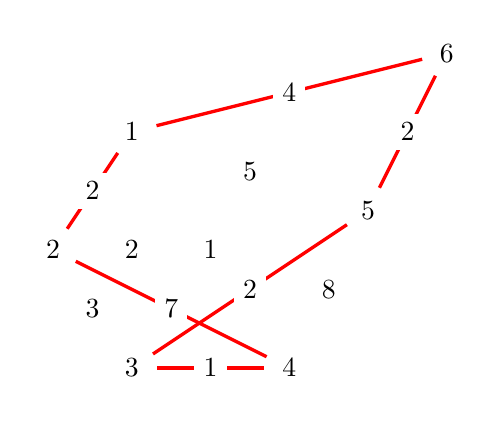
\begin{tikzpicture}
    \begin{scope}[every node/.style={circle,thick,draw=white,fill=white}]
        \node (3) at (1,0) {$3$};
        \node (2) at (0,1.5) {$2$};
        \node (1) at (1,3) {$1$};
        \node (4) at (3,0) {$4$};
        \node (5) at (4,2) {$5$};
        \node (6) at (5,4) {$6$};
    \end{scope}
    \begin{scope}[>={Stealth[black]},
        every node/.style={fill=white,rectangle},
        every edge/.style={draw=white,very thick}]%,
        \path [-] (1) edge[draw=red] node {2} (2);
        \path [-] (2) edge node {3} (3);
        \path [-] (1) edge node {2} (3);
        \path [-] (1) edge node {1} (4);
        \path [-] (1) edge node {5} (5);
        \path [-] (1) edge[draw=red] node {4} (6);
        \path [-] (2) edge[draw=red] node {7} (4);
        \path [-] (3) edge[draw=red] node {1} (4);
        \path [-] (3) edge[draw=red] node {2} (5);
        \path [-] (4) edge node {8} (5);
        \path [-] (5) edge[draw=red] node {2} (6);
    \end{scope}

\end{tikzpicture}
\end{document}
